\section{求解精度}
\label{sec:lpipm-accuracy}

内点法的迭代点永远在内部，算法只能在某一步停下来。这就需要回答：什么时候可以停，停下来的点能说明什么，以及如果需要的不是近似解而是一个基、甚至一张严格的证书，还要做什么？

\paragraph{三项残差共同决定停止}
一个点要接近最优，式~\eqref{eq:lpipm-kkt}的三组条件都要接近成立。通常用相对残差写成三条：
\begin{equation}
 \frac{\lVert\bm{A}\bm{x}-\bm{b}\rVert_2}{1+\lVert\bm{b}\rVert_2}\leq\varepsilon_{\mathrm{p}},\qquad
 \frac{\lVert\bm{A}^\top\bm{y}+\bm{s}-\bm{c}\rVert_2}{1+\lVert\bm{c}\rVert_2}\leq\varepsilon_{\mathrm{d}},\qquad
 \frac{\bm{x}^\top\bm{s}}{1+\lvert\bm{c}^\top\bm{x}\rvert}\leq\varepsilon_{\mathrm{g}}.
 \label{eq:lpipm-stop}
\end{equation}
分母里的$1$防止右端或目标恰好接近零时的除零。这些容差的意义依赖数据的尺度：把一条约束乘以$1000$，第一项的数值就改变，这和第~\ref{chap:optimization}章讨论可行性残差时指出的情况相同。

\paragraph{互补量何时是误差上界}
式~\eqref{eq:lpipm-gap-identity}的恒等式依赖两侧都可行，这时结论是干净的。

\begin{theorem}[可行点上的误差界]
\label{thm:lpipm-gap-bound}
设$\bm{x}$原始可行，$(\bm{y},\bm{s})$对偶可行。则
\begin{equation}
 0\leq\bm{c}^\top\bm{x}-p^\star\leq\bm{x}^\top\bm{s},\qquad
 0\leq d^\star-\bm{b}^\top\bm{y}\leq\bm{x}^\top\bm{s}.
 \label{eq:lpipm-gap-bound}
\end{equation}
\end{theorem}

\begin{proof}
$\bm{x}$可行给出$\bm{c}^\top\bm{x}\geq p^\star$。由弱对偶$\bm{b}^\top\bm{y}\leq d^\star\leq p^\star$，得到
\[
 \bm{c}^\top\bm{x}-p^\star\leq\bm{c}^\top\bm{x}-\bm{b}^\top\bm{y}=\bm{x}^\top\bm{s}.
\]
第二式同理，用$\bm{c}^\top\bm{x}\geq p^\star\geq d^\star$。
\end{proof}

两侧不可行时，这个界不再成立。此时
\[
 \bm{c}=\bm{A}^\top\bm{y}+\bm{s}-\bm{r}_{\mathrm{d}},\qquad\bm{b}=\bm{A}\bm{x}-\bm{r}_{\mathrm{p}}.
\]
代入目标差并整理，得到
\begin{equation}
 \bm{c}^\top\bm{x}-\bm{b}^\top\bm{y}=\bm{x}^\top\bm{s}-\bm{r}_{\mathrm{d}}^\top\bm{x}+\bm{r}_{\mathrm{p}}^\top\bm{y}.
 \label{eq:lpipm-gap-general}
\end{equation}

后两项的大小取决于残差和$\bm{x},\bm{y}$的大小。对目标误差有下面的两侧估计，它说明“残差小”换算成“目标差小”要付出什么。设$(\bm{x}^\star,\bm{y}^\star,\bm{s}^\star)$是一对最优解。

由$\bm{c}=\bm{A}^\top\bm{y}^\star+\bm{s}^\star$和$\bm{b}^\top\bm{y}^\star=p^\star$，直接计算得到
\[
 \bm{c}^\top\bm{x}-p^\star=(\bm{y}^\star)^\top\bm{r}_{\mathrm{p}}+(\bm{s}^\star)^\top\bm{x}\geq(\bm{y}^\star)^\top\bm{r}_{\mathrm{p}}.
\]
另一方面，把上面关于$\bm{c}$的表达式用到最优解$\bm{x}^\star$上，得到
\[
 p^\star=\bm{c}^\top\bm{x}^\star=\bm{b}^\top\bm{y}+\bm{s}^\top\bm{x}^\star-\bm{r}_{\mathrm{d}}^\top\bm{x}^\star.
\]
由$\bm{s}^\top\bm{x}^\star\geq0$和式~\eqref{eq:lpipm-gap-general}，得到上界。合起来就是
\begin{equation}
 (\bm{y}^\star)^\top\bm{r}_{\mathrm{p}}
 \leq\bm{c}^\top\bm{x}-p^\star
 \leq\bm{x}^\top\bm{s}+\bm{r}_{\mathrm{p}}^\top\bm{y}+\bm{r}_{\mathrm{d}}^\top(\bm{x}^\star-\bm{x}).
 \label{eq:lpipm-near-bound}
\end{equation}

这个结果的含义是，等式残差被最优解的大小放大。左端里$\bm{y}^\star$相当于影子价格：原始残差$\bm{r}_{\mathrm{p}}$相当于多用了或少用了资源，目标可以因此偏离$(\bm{y}^\star)^\top\bm{r}_{\mathrm{p}}$。所以$\bm{x}^\top\bm{s}$小并不代表目标差小，还要等式残差足够小。

图~\ref{fig:lpipm-gap-sandwich}展示了这种差别。图(a)的起点严格可行，蓝线$\bm{c}^\top\bm{x}$从上方、紫线$\bm{b}^\top\bm{y}$从下方夹住$p^\star=1$，这就是定理~\ref{thm:lpipm-gap-bound}。图(b)的起点是$\bm{x}=0.1\bm{1}$、$\bm{s}=\bm{1}$、$y=0$，等式不成立，蓝线一度在红线下方，说明此时目标值比最优值还小，并不是好事，这和第~\ref{chap:optimization}章资源分配中那个超出资源的点是同一种现象。

\begin{BookInlineFigure}
  \centering
  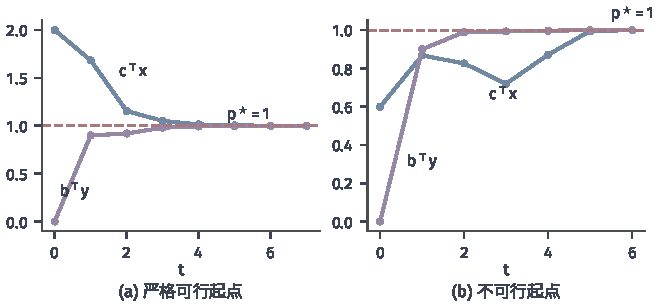
\includegraphics[width=112mm]{figures/05-optimization/01-linear-programming/matplotlib/lpipm-gap-sandwich/figure.pdf}
  \caption{原始目标（蓝）与对偶目标（紫）的夹逼，红色虚线是$p^\star=1$，$\sigma=0.3$。(a)严格可行起点，两条线从两侧夹住最优值，差距等于$\bm{x}^\top\bm{s}$。(b)不可行起点$\bm{x}=0.1\bm{1}$、$\bm{s}=\bm{1}$、$y=0$，前几轮原始目标低于最优值，原始目标甚至低于对偶目标。}
  \label{fig:lpipm-gap-sandwich}
\end{BookInlineFigure}

用图(b)的第一轮结果核对。那一点的数据是
\[
 \bm{x}\approx(0.1744,0.1521,0.1298)^\top,\qquad y=0.9,\qquad\bm{s}\approx(0.1,0.3231,0.5463)^\top,
\]
等式残差和目标值是
\[
 r_{\mathrm{p}}\approx-0.5438,\qquad\bm{r}_{\mathrm{d}}\approx(0,-0.7769,-1.5537)^\top,\qquad\bm{c}^\top\bm{x}\approx0.8678.
\]
这时$\bm{x}^\top\bm{s}\approx0.1375$是正的，但$\bm{c}^\top\bm{x}-\bm{b}^\top\bm{y}\approx-0.0322$是负的，与式~\eqref{eq:lpipm-gap-general}的右端一致。

目标误差$\bm{c}^\top\bm{x}-p^\star\approx-0.1322$落在式~\eqref{eq:lpipm-near-bound}的两端之间：左端$y^\star r_{\mathrm{p}}\approx-0.5438$，右端约为$-0.0322$。

\paragraph{近似解与精确解}
停止时得到的点满足式~\eqref{eq:lpipm-stop}，这是在给定容差和浮点运算下的结论。它和精确最优解是两回事，具体差别至少有三处。

第一，它通常不可行：$\bm{A}\bm{x}=\bm{b}$只成立到舍入误差，$\bm{x}>\bm{0}$只在严格的算术上成立。第二，它不是顶点：贯穿例第$7$轮的$x_2,x_3$是$2\times10^{-4}$和$1\times10^{-4}$，并不是零，把它们置零之后等式又不成立了。第三，浮点解的最后几位受舍入和$\bm{M}$的条件数影响，容差设得过小并不会让结果更准，反而可能使线性系统求解失败。

所以报告结果时应当把三项残差一起报告，说明容差和尺度。“求解成功”指的只是这三项达标，至于是否足够精确，要看用途。

\paragraph{基恢复}
有些用途需要一个基：要接着用单纯形法作参数分析（第~\ref{chap:simplex-method}章），要作整数规划的分支，或者需要一个顶点解。内点法不直接给出基，要从近似解转换，这一过程称为\term{基恢复}（crossover）。

做法分两阶段。先由$\hat{\bm{x}}$和$\hat{\bm{s}}$猜测哪些变量为正，例如比较$\hat{x}_i$与$\hat{s}_i$的大小，把判为零的$x_i$置零，并在其余列上修正使等式成立。然后，判为正的变量可能多于$m$个，这时沿$\bm{A}$的零空间方向移动，保持目标不变并把多余的变量逐个推到零，直到剩下的列线性无关；对偶一侧作类似的推动。最后得到一个基，用单纯形法的计算重新求出解并检查符号。

以第~\ref{sec:lpipm-central-path}节目标$\bm{c}=(0,0,1)$的例子说明。设内点法输出近似解$\hat{\bm{x}}=(0.4995,0.4995,0.001)^\top$，$\hat{\bm{s}}$的前两个分量很小，第三个分量接近$1$。比较大小后判定$x_3=0$，并修正成$(1/2,1/2,0)^\top$。

正的变量有两个，而$m=1$，还多一个。沿零空间方向$\bm{d}=(1,-1,0)^\top$移动，目标不变，走到$x_2=0$，得到顶点$(1,0,0)^\top$，基是$B=(1)$，如图~\ref{fig:lpipm-crossover}。

\begin{BookInlineFigure}
  \centering
  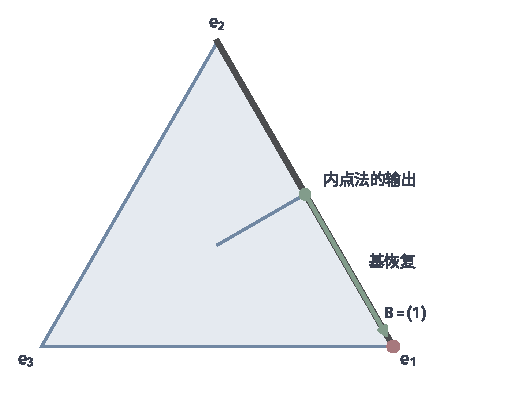
\includegraphics[width=90mm]{figures/05-optimization/01-linear-programming/matplotlib/lpipm-crossover/figure.pdf}
  \caption{基恢复的一步。目标$\bm{c}=(0,0,1)$，深灰粗线是最优边，蓝线是中心路径。内点法的输出（绿点）靠近最优边的中点，沿最优边的方向推到端点$\bm{e}_1$（红点），得到基$B=(1)$。推向$\bm{e}_2$同样得到一个最优基，所以恢复的基不唯一。}
  \label{fig:lpipm-crossover}
\end{BookInlineFigure}

用这个基作检验。$\bm{x}_B=1$，对偶是$\bm{y}=\bm{A}_B^{-\top}c_1=0$，约化成本是
\[
 \bm{s}=\bm{c}-\bm{A}^\top\bm{y}=(0,0,1)^\top\geq\bm{0},
\]
基是最优的。如果符号检验失败，从这个基继续作若干次单纯形换基。基恢复的工作量取决于$\hat{\bm{x}}$的正分量比$m$多多少，以及猜测的准确程度。已知严格互补解时恢复最优基只需多项式次运算，但实际耗时可能超过内点迭代本身。

\paragraph{精确证书}
基恢复之后得到的基和解还是浮点数算出的。如果数据是有理数，又需要严格证书，要再走一步。基矩阵$\bm{A}_B$本身是精确的，所以可以用有理数运算重新计算
\begin{equation}
 \bm{x}_B=\bm{A}_B^{-1}\bm{b},\qquad\bm{y}=\bm{A}_B^{-\top}\bm{c}_B,\qquad\bm{s}=\bm{c}-\bm{A}^\top\bm{y},
 \label{eq:lpipm-exact-check}
\end{equation}
并精确地检查$\bm{x}_B\geq\bm{0}$和$\bm{s}\geq\bm{0}$。这种检查不受任何舍入影响，通过时就是严格的最优性证明，这一点和第~\ref{chap:linear-programming}章的证书完全一致。

另一种办法是先把浮点解有理化，再验算。由Cramer法则，基本解的分母整除$\det\bm{A}_B$。两个分母都不超过$Q$的不同有理数至少相差$1/Q^2$，所以浮点解的误差只要小于$1/(2Q^2)$，分母不超过$Q$的最近有理数就只有一个，可以通过连分数求出，然后再用精确运算核对。

例如把贯穿例的约束改成$3x_1+x_2+x_3=1$，最优解是$x_1=1/3$。设内点法和基恢复给出$\hat{x}_1=0.33333341$。这里$\det\bm{A}_B=3$，分母不超过$3$的最近有理数是$1/3$。在基$B=(1)$上按式~\eqref{eq:lpipm-exact-check}作精确计算，得到
\[
 x_1=\frac13,\qquad y=\frac13,\qquad\bm{s}=\Bigl(0,\frac53,\frac83\Bigr)^\top\geq\bm{0}.
\]
这是一张可以逐项核对的最优性证书。

图~\ref{fig:lpipm-solution-pipeline}把这几个阶段连起来。算法名义上“求解完成”可以停在其中任何一个阶段，每一阶段交出的东西含义不同：近似的内部点、一个基、一个浮点最优性检验通过的基、一张严格的证书。使用结果时要分清拿到的是哪一种。

\begin{BookInlineFigure}
  \centering
  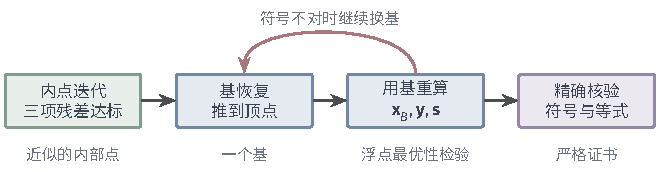
\includegraphics[width=111.739mm]{figures/05-optimization/01-linear-programming/tikz/lpipm-solution-pipeline/figure.pdf}
  \caption{从内点迭代到严格证书的各个阶段。下方灰字是每个阶段交出的结果，红色箭头表示基恢复后符号检验不通过时继续换基。}
  \label{fig:lpipm-solution-pipeline}
\end{BookInlineFigure}
